\chapter{Un ejemplo de R H Bing}

Ejemplo: Una 2-esfera salvaje $S$ y una curva cerrada simple $J\subset\R^3-S$ tales que 
\begin{itemize}
    \item $J$ no es trivial en $\R^3-S$
    \item Para todo disco $D\subset S$, $J$ es trivial en $\R^3-D$
\end{itemize}
              
Partimos de $S_0$ una esfera domesticada. 

Sea $E_1,\dots,E_n$ una descomposición celular de $S_0$ \comm{definir} tal que $E_i$ y $E_{i+1}$ comparten borde para todo $i\in\{1,\dots,n-1\}$, y $E_1$, $E_n$ también compartan borde. 

Engordamos las células $E_i$ \duda{¿qué debería decir? tomar entorno tubular? tendría que definir mejor esto} y les agregamos un cilindro con un asa al final $H_i$ para obtener un toro $T_i$, de manera que el agujero de $T_i$ encierre al cilindro de $H_{i+1}$. De la misma manera $H_n$ encierra el cilindro de $H_1$. 
            
Consideramos $H_i$ toros sólidos, a los que nos referiremos como "lazos", y tomamos $E_i'$ un entorno tubular de $E_i$. 
            
Definimos $T_i$ como el pegado de $E_i'$ con $H_i$ por un disco, de manera que el agujero de $H_i$ encierre a $T_{i+1}$ como se ve en la imagen. 

Más específicamente, consideramos una 2-célula $C_i$ y pegamos $\partial C_i$ con $\gamma_i\subset T_i$ una curva no contractible en $T_i$, llamamos a este pegado $T_i'$. 
            
Ahora colapsamos $C_i$, es decir, cocientamos $T_i'$ por la relación $x\sim y \Leftrightarrow x,y\in C_i$. Definimos el pegado de arriba de manera que, al hacer este colapso, el cociente de $T_{i+1}$ tenga dos componentes conexas: una que contiene a $E_{i+1}'$ y otra que es un toro.

Llamamos $W_1=\bigcup\limits_{i=1}^n T_i$. 

La 2-esfera $S$ del ejemplo va a estar contenida en $W_1$, y va a intersectar a $\bigcup\limits_{i=1}^n\partial T_i$ sólamente en $\bigcup\limits_{i=1}^n\partial E_i$.

\begin{figure}[h!]
    \centering
    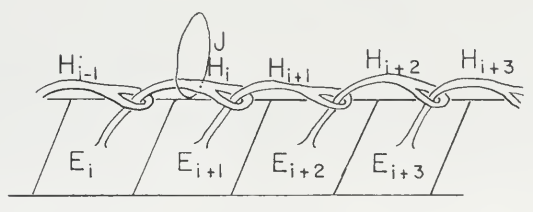
\includegraphics[width=0.5\linewidth]{img mono/hooked rug/1.png}
    \caption{$J$ no trivial en $W_i$}
    \label{hr1}
\end{figure}
            
Por el teo 11 una curva $J$ como en la imagen es no trivial en $\R^3-W_1$ \comm{justificar mejor} 

Ahora sacamos un cilindro sólido de cada $H_i$ para obtener un cubo topológico $K_i$. \duda{cubo topológico? por qué no decir esfera sólida/bola? yo le copié al bing}

Observar que $\partial E_i$ divide $\partial K_i$ en dos discos, uno que está contenido en la componente acotada de $\R^3-S_0$ y otro que está contenido en $H_i$ pero que ya no encierra a $H_{i+1}$. 
            
Llamamos a este segundo disco $D_i$.  
          
Movemos homotópicamente el interior de este segundo disco de manera que quede contenido en $int(T_i)$. Entonces tenemos $D_i\subset int(T_i)$ y $\partial D_i=\partial E_i$. 

Luego $\bigcup\limits_{i=1}^n D_i$ es una esfera, a la que llamamos $S_1$. 

Ahora subdividimos cada $D_i$ en 2-células $E^i_1,\dots, E^i_{15}$ tal que $E^{i}_{j},E^{i}_{j+1}$ comparten borde para todo $i\in\{1,\dots,14\}$, $E^{i}_{15}$ y $E^{i}_{1}$ compartan borde. \duda{q pasa si usamos otros números? obtenemos esferas no equivalentes supongo. y qué pasa si usamos x ejemplo n=2? funciona igual?} 

Continuamos con un proceso similar. Ahora engordamos los $E^i_j$ y les pegamos un toro $H_i$ por un disco para formar un toro sólido $T^i_j$, que de la misma manera que antes encierra a $T^i_{j+1}$ para todo $j\in\{1,\dots, 14\}$, y $T^i_{15}$ encierra a $T^i_1$.  
            
Además pedimos que dos cilindros de $T^i_j$ no consecutivos, por ejemplo $T^i_7$ y $T^i_{11}$, se enrieden como en la siguiente imagen: \duda{no me queda claro si pedir q no sean consecutivos es lo único que se necesita}

\begin{figure}[h!]
    \centering
    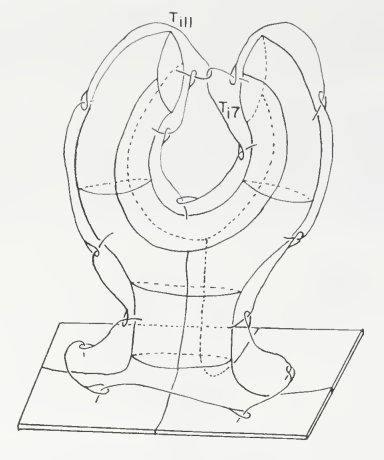
\includegraphics[width=0.5\linewidth]{img mono/hooked rug/2.png}
    \caption{$T^i_j$ se enriedan}
    \label{hr2}
\end{figure}

Por los teoremas 9 y 11 tenemos que cualquier curva cerrada no trivial en $\R^3 - T_i$ es no trivial en $\R^3-\sum T^i_j$. \comm{justificar}
            
Hacemos esta construcción de manera que $\bigcup\limits_{j=1}^{15} T^i_j\subset T^i$, es decir, tomamos los $T^i_j$ bien pegaditos a los $E^i_j$. (También puedo decir que están bien pegaditos al $D_i$) 

De la misma forma que antes, sacamos un cilindro sólido de cada $T^i_j$ para obtener un cubo $K^i_j$, cuyo borde es separado en dos discos por $\partial E^i_j$. Llamamos $D^i_j$ al disco contenido en la componente conexa de $T^i_j-E^i_J$ que es un toro, y movemos $int(D_j^i)$ mediante una homotopía para que quede contenido en $int(T_j^i)$. 

Llamamos entonces $S_2$ a la esfera $\bigcup\limits_{i,j} D^i_j$. También llamamos $W_2$ a $\bigcup\limits_{i,j}T^i_j$ 

El ejemplo $S$ es el límite de la secuencia $\{S_i\}_{i\in\N}$, y también es $S=\bigcap\limits_{i\in\N}W_i$, con $W_i$ 3-variedades con borde. \duda{ustificar por qué la secuencia tiene límite y cómo defino eso y tb justificar por qué la intersección de los $W_i$ es una variedad sin borde.}

En general, para obtener $S_{n+1}$ y $W_{n+1}$ a partir de $S_n=\bigcup\limits_{i=1}^{15}D_i$ y $W_n=\bigcup\limits_{i=1}^{15}T_i$ el proceso es el siguiente: 
            
Subdividimos cada disco $D_i$ de la construcción de $S_n$ en 15 discos que llamaremos $E^i_1,\dots, E^i_{15}$, luego tomamos sus entornos tubulares $E^{i'}_{j}$ y los pegamos con un toro $H_j^i$ por un disco, obteniendo toros $T^i_1,\dots,T^i_{15}$ de manera que queden enganchados como describimos antes, y de manera que dos lazos $T_j^i$ y $T_k^i$ no consecutivos se enrieden entre sí como se mostraba en la imagen. 
            
Además nos aseguramos de tomar estos $T_j^i$ bien cerca de $D_i$ para que $\bigcup\limits_{j} T^i_j\subset T_i$

La 3-variedad con borde $W_{n+1}$ la definimos como $\bigcup\limits_{i,j} T_j^i$ y cumple $W_{n+1}\subset W_n$. 

Después sacamos un cilindro de cada uno de los toros $T_j^i$ para obtener cubos $K_j^i$, que son separados por $\partial E_j^i$ en dos discos. 

Llamamos $D_j^i$ al disco contenido en la componente conexa de $T_j^i - E_j^i$ que es un toro, y movemos $int(D_j^i)$ mediante una homotopía para que quede contenido en $int(T_j^i)$. 

Definimos $S_{n+1} = \bigcup\limits_{i,j} D_j^i$. 

¿Por qué este límite es una esfera?

Sea $S_n=\bigcup D_i$ como en la construcción, entonces $\partial D_i\subset S_{n+k} \fall k\in\N \Rightarrow \partial D_i\subset \lim\limits_{n\to\infty} S_n$ 

Además, dados $D_{i_1},D_{i_2}$ discos de la construcción de $S_n$, se tiene que $D_{i_1}\cap D_{i_2}=\varnothing$ y como $D_i\subset W_n$ y sus subsecuentes modificaciones van a seguir estando en $W_{n+k}$ y por lo tanto las modificaciones no se van a intersectar. \duda{r h what are you trying to tell me} 

\begin{figure}[h!]
    \centering
    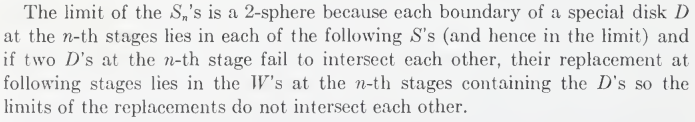
\includegraphics[width=0.5\linewidth]{img mono/hooked rug/esfera.png}
    \caption{tengo que escribir bien esto}
    \label{esfera}
\end{figure}

Entre cada $S_n, S_{n+1}$ tenemos un homeo $h_n$ \comm{escribirlo explícitamente}

Si definimos estos homeos para que $\{f_n=h_n\circ\dots\circ h_0\}_{n\in\N}$ converjan uniformemente, entonces existe el límite $f:S_0\to S$ y es continua. 

Si $f$ fuera biyectiva entonces sería un homeo porque $S_0$ compacto y $S$ es Hausdorff \comm{poner prueba de esto y de por qué S es hff}
 

$\textbf{Afirmación:}$ Si $J$ es una curva cerrada simple como en la primer imagen, entonces $J$ no es homotópica a un punto en $\R^3 - S$ 

\begin{dem}
          
$J\sim\ast$ en $\s^c \Rightarrow J\sim\ast$ en $(\bigcap\limits_{i\in\N} W_i)^c\Rightarrow J\sim\ast$ en $\bigcup\limits_{i\in\N} W_i^c\Rightarrow J\sim\ast$ en algún $W_i^c$

Veamos que tener una homotopía de $J$ a un punto en algún $W_i^c$ es absurdo. 

Sea $W_i'$ el conjunto obtenido rellenando los agujeros de $W_i$ \duda{me parece raro decir esto así}, entonces $W_i'$ es una esfera \comm{o una "bola hueca" porque en realidad estamos tomando un entorno tubular del borde, pero no sé si importa decir esto} con manijas y sea $W_i''$ el conjunto obtenido quitando un cilindro de cada agujero en $W_i$ \duda{también esto xd y no entendí lo que sigue} \end{dem}

\begin{teo}{Teorema 9} Sea $C$ un cilindro con bases $B_1$ y $B_2$, sean $T_1,\; T_2$ dos toros enganchados entre sí \duda{se puede decir así esto?} tales que $T_i\cap\partial C=B_i$ y sea $X\subset\R^3$ un cerrado tal que $X\cap C=B_1\cup B_2$. 
          
Entonces, dada una curva simple y cerrada $J \subset (X\cup C)^c$, tenemos que $J$ no es homotópica a un punto en $(X\cup T_1\cup T_2)^c$ \end{teo}

\begin{figure}[h!]
    \centering
    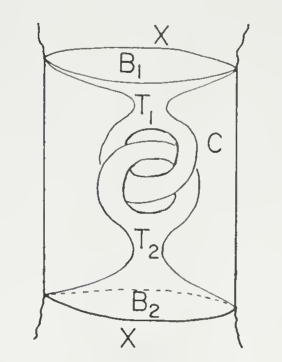
\includegraphics[width=0.5\linewidth]{img mono/hooked rug/3.png}
    \label{hr3}
\end{figure}

\begin{teo}{Teorema 11} Sean $C$ un cubo topológico, $B_1,\; B_2,\; B_3\subset\partial C$ discos disjuntos dos a dos, $C_1$ cubo topológico tal que $C_1\cap int(C)^c =B_1\cup B_2$, $T$ un toro sólido tal que $T\cap C=B_3$ y tal que $T$ engancha $C_1$. 

Sea $X$ un cerrado tal que $X\cap C= B_1\cup B_2\cup B_3$ y tal que $\partial B_i$ no es homotópico a un punto en $\partial B_i \cup (X\cup C)^c$ para $i=1,\;2$. 

Entonces, si $J$ es una curva simple cerrada en $(X\cup C)^c$ y no es homotópica a un punto en $(X\cup C)^c$, se tiene que $J$ no es homotópica a un punto en $(X\cup C_1\cup T)^c$. \end{teo}

\begin{figure}[h!]
    \centering
    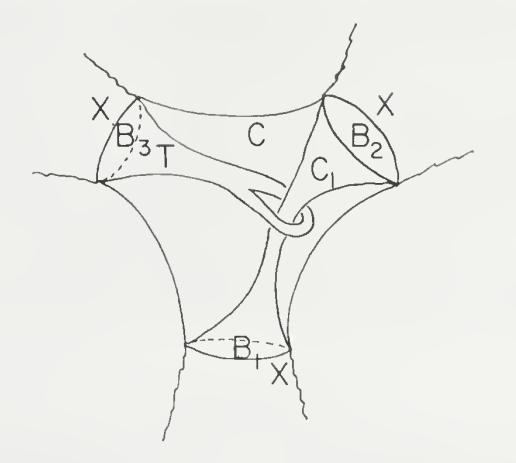
\includegraphics[width=0.5\linewidth]{img mono/hooked rug/4.png}
    \label{hr4}
\end{figure}